\section{Motivation}
\label{sec:motivation}
In this section, we first motivate our work by showing how a model can be compiled in different ways
and subsequently, show the drastic performance difference across these variants for real benchmarks.

\subsection{Motivating Example}
\begin{figure}[htb]
  \centering
  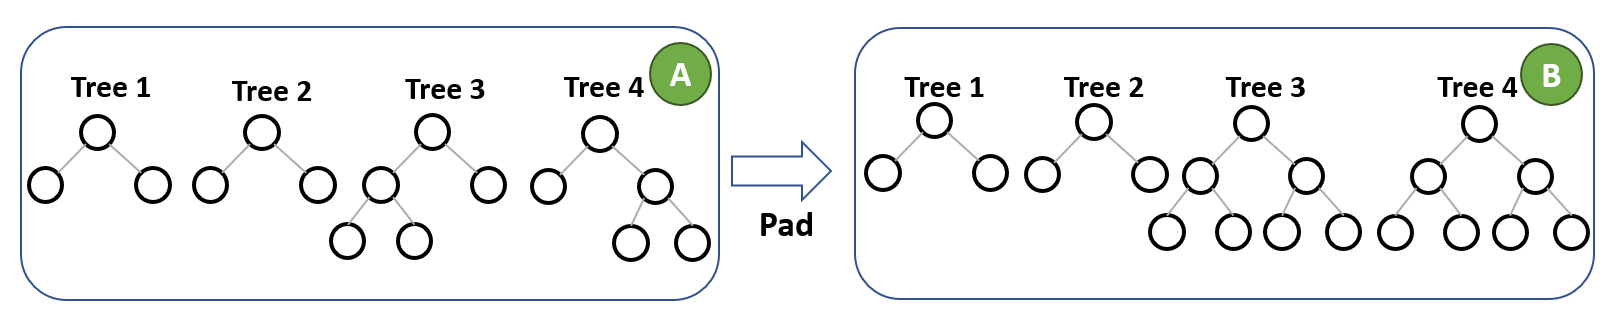
\includegraphics[width=\linewidth]{figures/HIR.PNG}
  \caption{Model for motivating example. The model has four trees, two of depth 1 and two of depth 2.}
  \label{Fig:HIRExample}
\end{figure}

Consider a model with four trees, two 
trees of depth 1 and two of depth 2 (\circled{A} in Figure \ref{Fig:HIRExample}).
% We use this model as our running example throughout this section.
We first describe the simple schedule shown in Figure \ref{fig:schedulea} that processes one tree at a time 
for all input rows\footnote{Since the scheduling constructs are fairly intuitive, we 
defer a detailed explanation of the scheduling language to Section~\ref{sec:schedule}.}.
In this schedule, the loop over the trees is split into two -- one that
iterates over the first two trees (Trees 1 and 2 with depth 1) and 
the second that iterates over the last two trees (Trees 3 and 4 with
depth 2). Straightforward traversal of trees requires a \op{while} loop
and involves branching to check if a leaf has been reached. 
One way to avoid this, as done in this schedule, is to unroll the 
tree walks for each tree. 
When the schedule specifies that the tree walks should be unrolled, 
\Treebeard{} pads the trees so that all leaves of a tree are at the same depth
(\circled{B} in Figure~\ref{Fig:HIRExample}). 
The concrete implementation of this schedule (in \Treebeard{}'s IR) 
is as shown in Figure \ref{fig:schedulea}\footnote{We do not show 
the full listing of the IR. Instead, we present inference routines 
as pseudo-code for the sake of clarity.}.
This schedule is ideally suited for a single-core CPU. It maximizes 
the reuse of trees in the L1 cache. However, it doesn't exploit  
any parallelism. 

\begin{figure*}[]
  \begin{subfigure}[t]{.5\linewidth}
    \vspace{0pt}
    \centering
    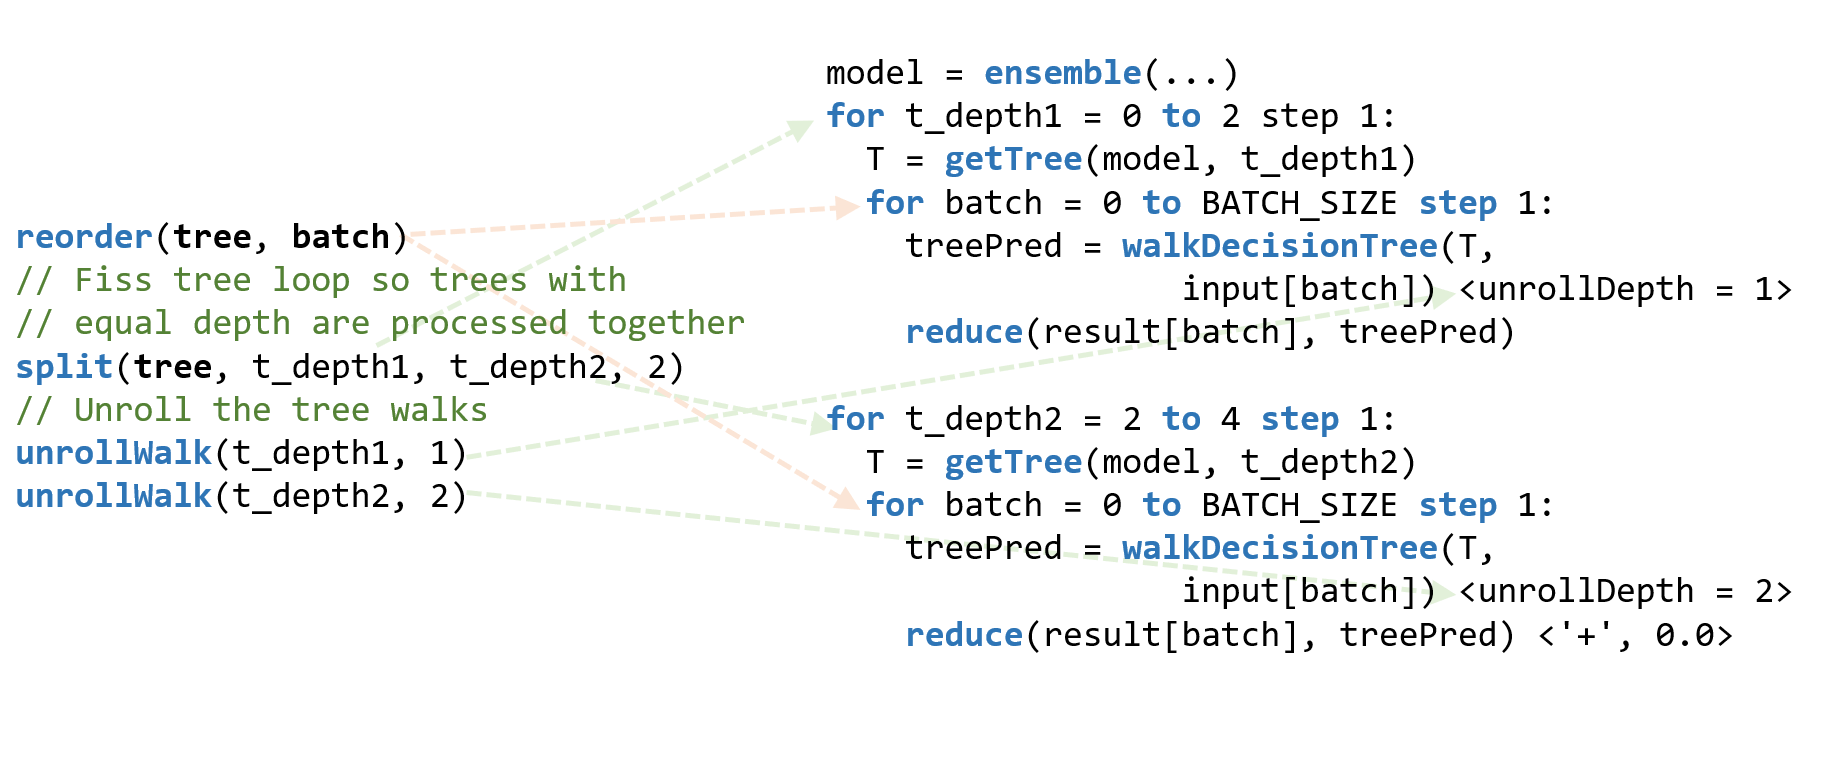
\includegraphics[width=\linewidth]{figures/MotivatingExample1.PNG}
    \caption{\label{fig:schedulea}}
  \end{subfigure}\hfill
  \begin{subfigure}[t]{.5\linewidth}
    \vspace{0pt}
    \centering
    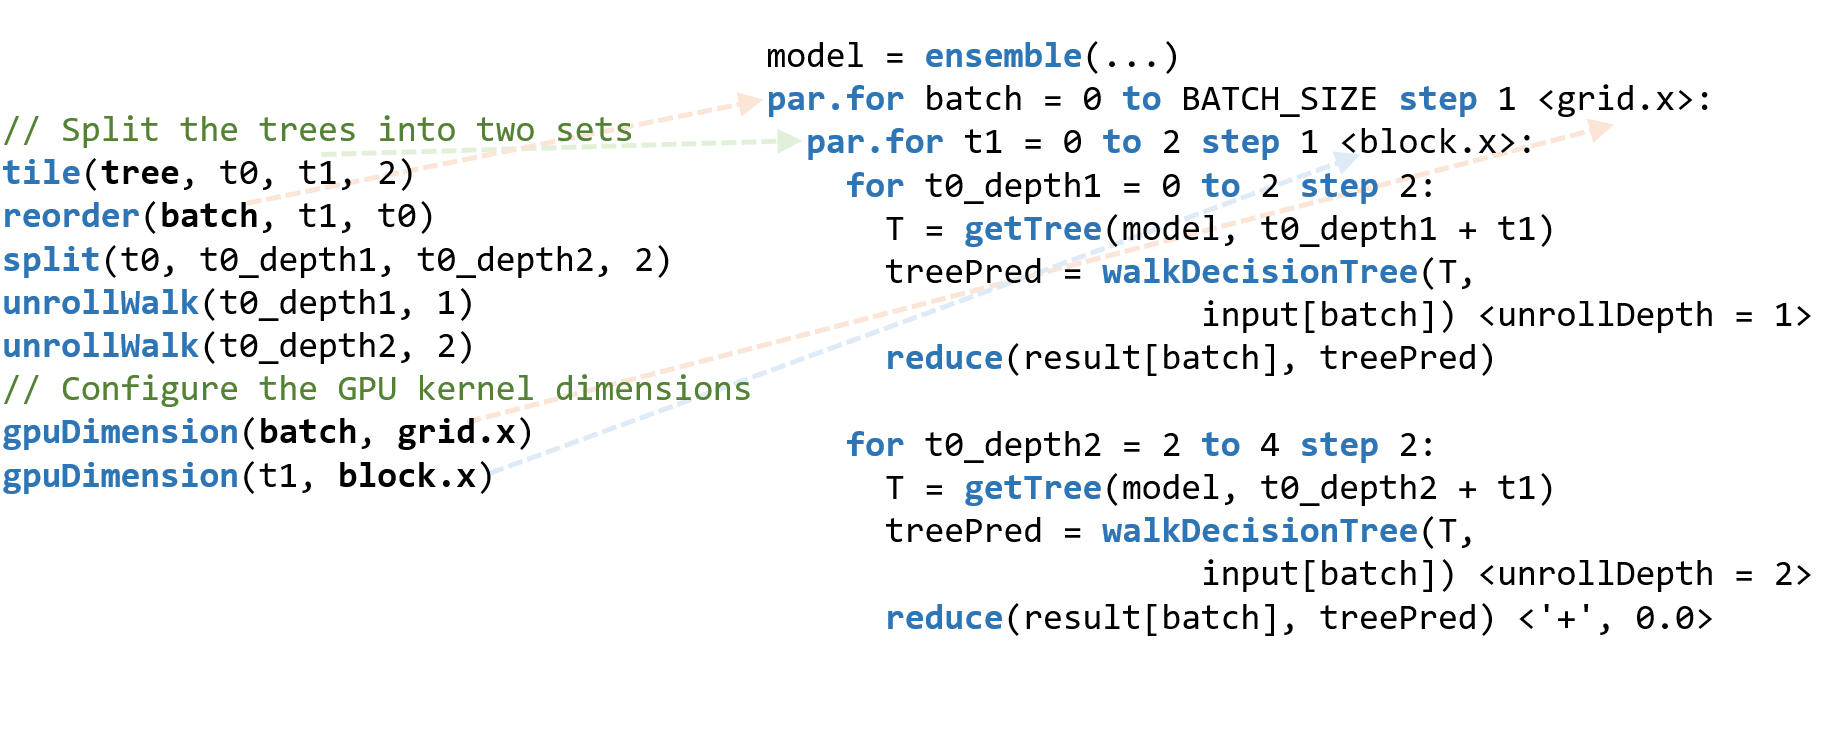
\includegraphics[width=\linewidth]{figures/MotivatingExample2.PNG}
    \caption{\label{fig:scheduleb}}
  \end{subfigure}
  \caption{Some possible schedules to compile the motivating example and the generated \Treebeard{} IR.
  The arrows connect entities in the schedule to related entities in the IR. }
  \label{Fig:Schedules}
\end{figure*}

One form of parallelism that can be exploited is to process rows in parallel. 
While this may work for multi-core CPUs\footnote{As we report in Section~\ref{sec:results}, 
other ways to parallelize can benefit inference on CPUs as well.}, with massively parallel processors like GPUs,
 this strategy may not yield sufficient parallel work. To expose more parallelism, 
we can additionally parallelize across trees as done in the schedule in Figure \ref{fig:scheduleb}. 
The corresponding GPU inference routine is shown in the same figure. 
This schedule generates a routine that processes one input row per thread block (\op{batch}
loop is mapped to \op{grid.x}). The schedule also tiles the \op{tree} loop into a
nest of two loops with indices $t0$ and $t1$. It then additionally parallelizes across the $t1$ loop.
Finally, it splits $t0$ and unrolls the walks for each tree depth.

Note that while unrolling helps avoid branching, it increases 
the total amount of computation. Another option is to not unroll 
and let the GPU manage the branching. The schedules with and 
without unrolling place different constraints on the target processor,
and the best choice depends on the characteristics of the model
and micro-architectural features like register file size and handling 
of branch divergence~\cite{FungMicro, MilindDivergence}.

These \Treebeard{} schedules just use a combination of 4-8 constructs and already generate strategies 
that are different from what library based systems like XGBoost, Tahoe and RAPIDs FIL use. 
As one can imagine, several other schedules with different trade-offs can be generated using 
these constructs.

\subsection{Performance of Different Schedules} 
\begin{figure}[htb]
  \begin{subfigure}[t]{.45\linewidth}
    \vspace{0pt}
    \centering
    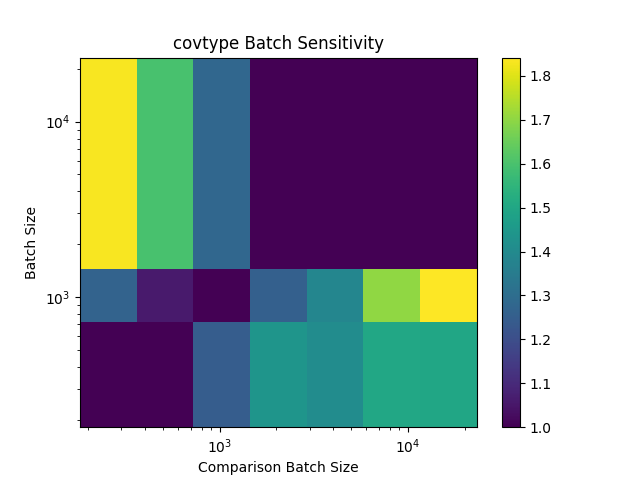
\includegraphics[width=\linewidth]{figures/batch_sensitivity_covtype.png}
    \vspace{2pt}
    \caption{\label{fig:sensitivitya}\op{covtype} batch sensitivity}
  \end{subfigure}\hfill
  \begin{subfigure}[t]{.52\linewidth}
    \vspace{0pt}
    \centering
    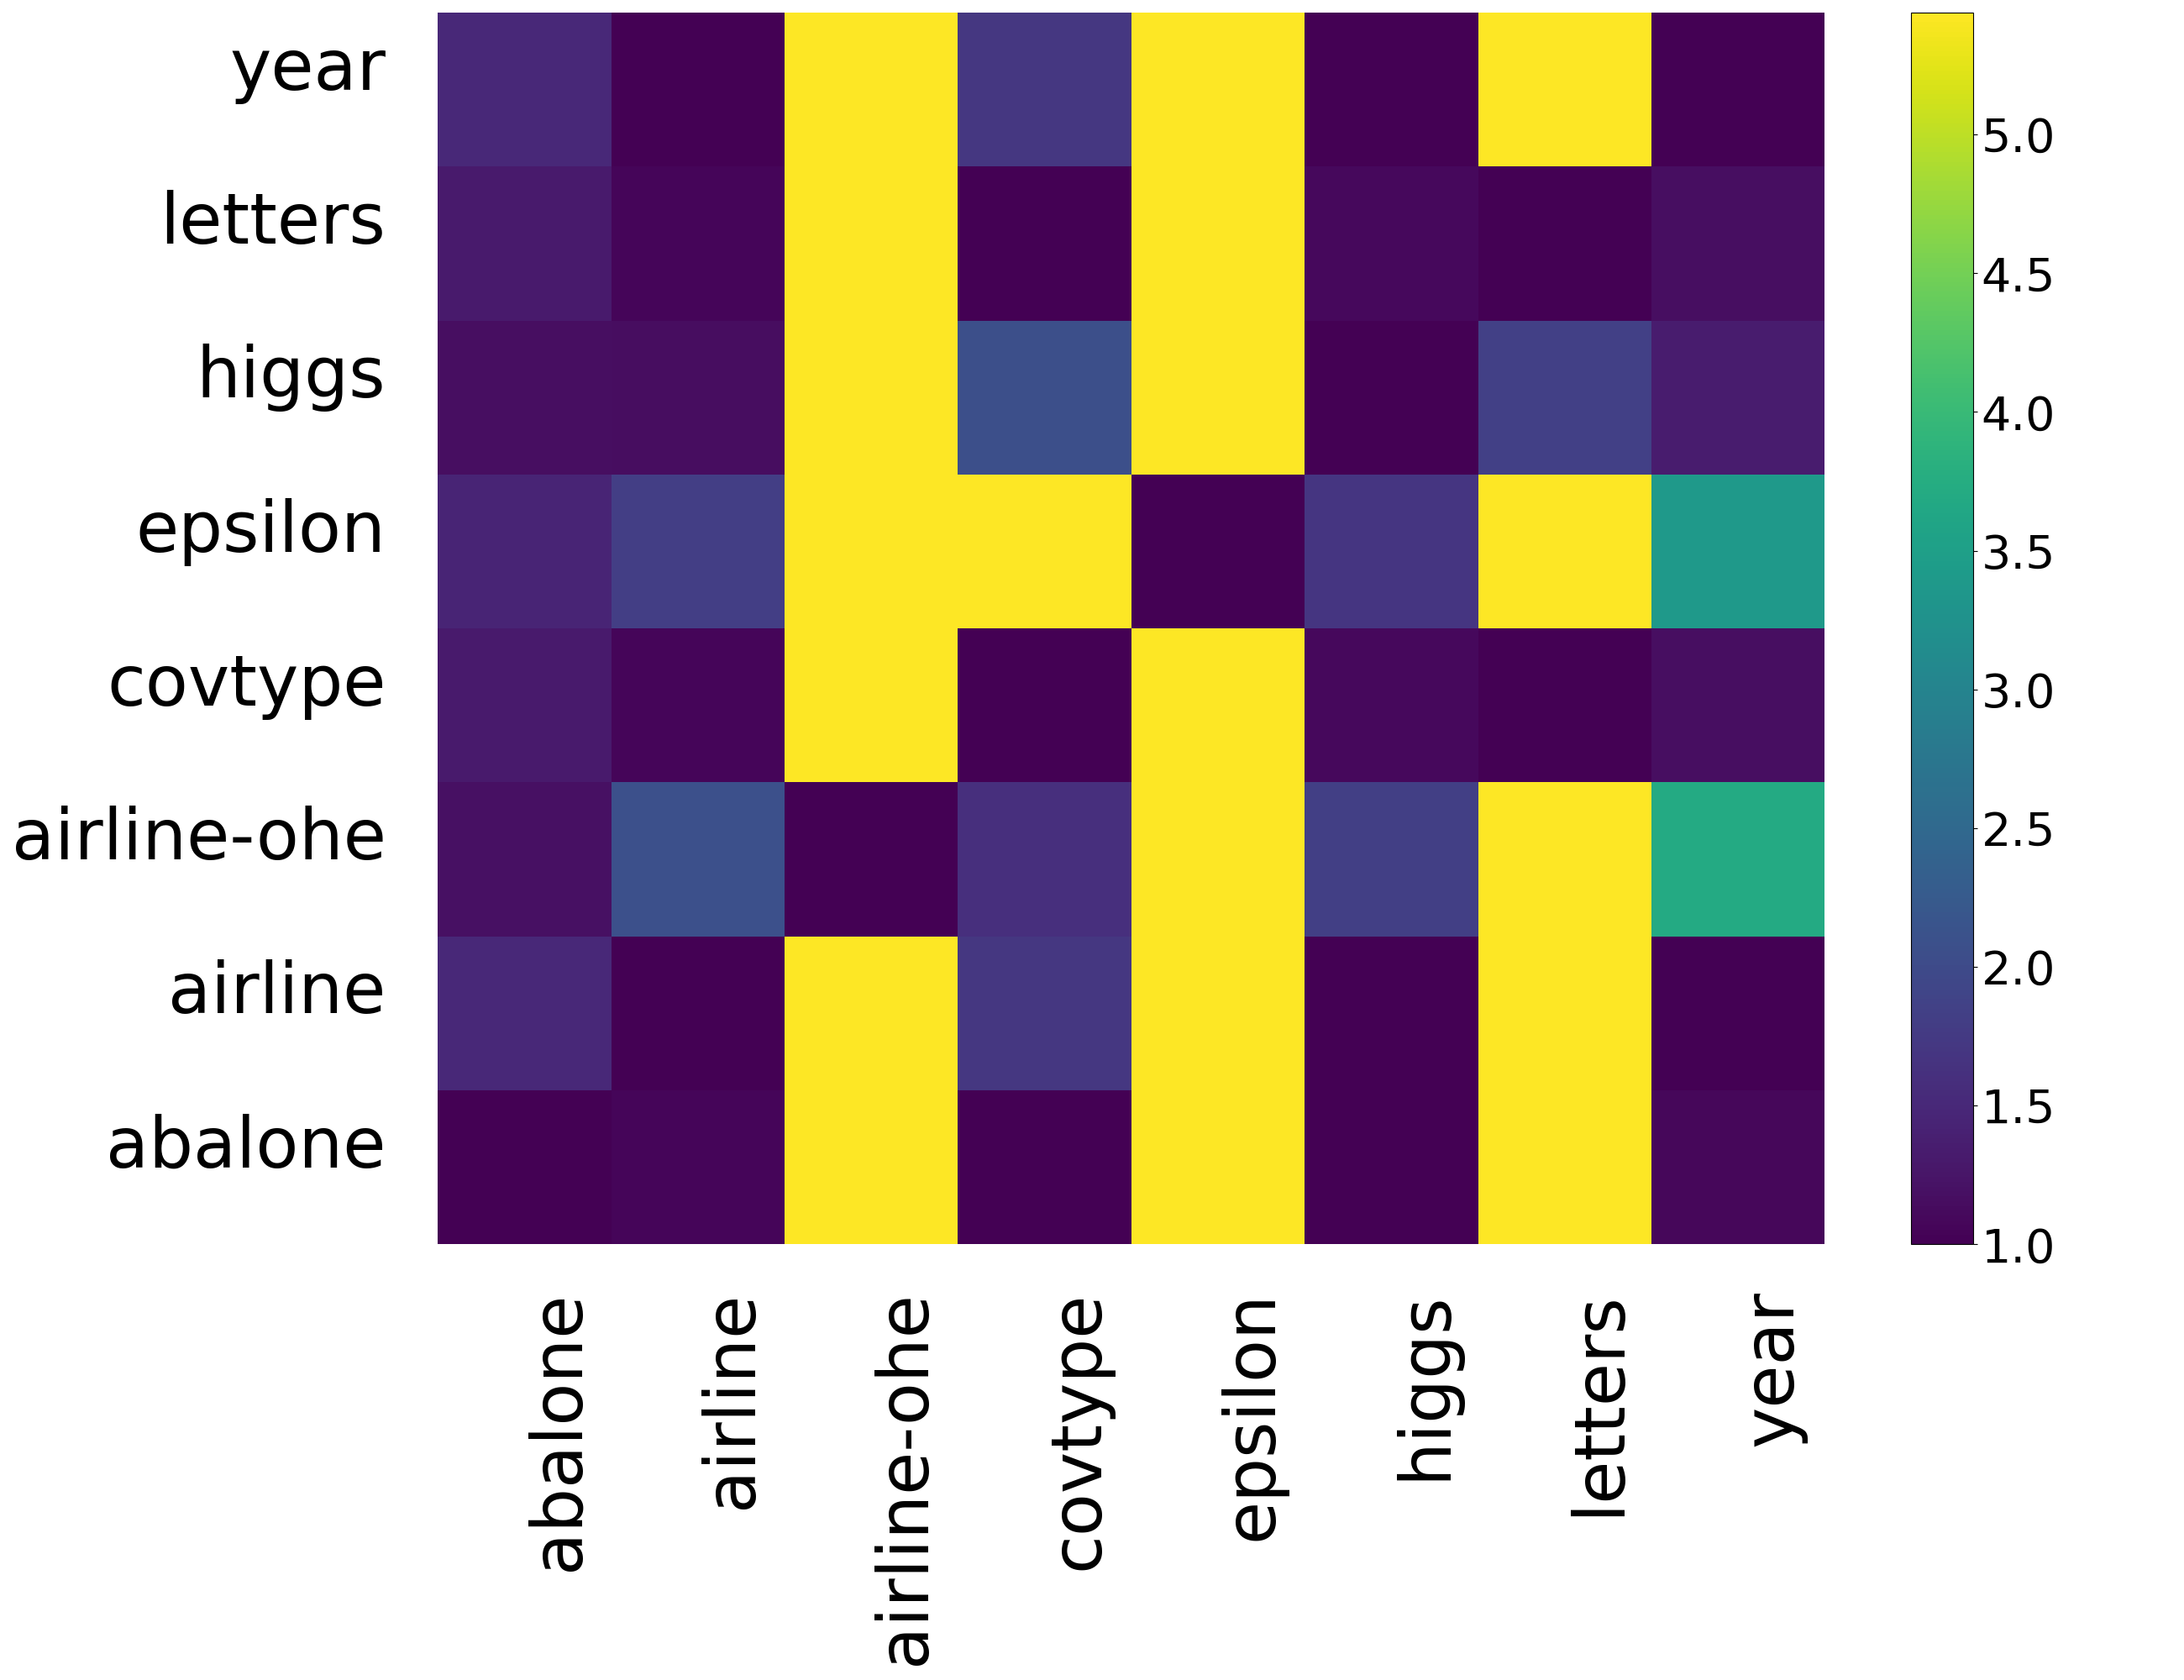
\includegraphics[width=\linewidth]{figures/model_sensitivity_4096.png}
    \caption{\label{fig:sensitivityb}Model sensitivity at batch size 4096}
  \end{subfigure}
  \caption{Batch and model sensitivity plots. Each point shows the slowdown when the best 
  schedule for the x-axis batch size (model) is used for the y-axis batch size (model).}
\end{figure}

To establish the importance of choosing the right schedule, we
compare the performance of the schedules generated by \Treebeard{}
on several real-world benchmarks. 
Figure~\ref{fig:sensitivitya} shows the
variation in performance when the best schedule for a given batch 
size is used across different batch sizes for one of the models. 
Figure~\ref{fig:sensitivityb} shows the variation when schedules 
are used across models at a fixed batch size.
% These diagrams show that the best schedules to use vary across batch sizes and models. 
As can be seen, performance degrades by 2$\times$ when the best schedule for a
smaller batch size is used for a larger batch size and vice-versa.
Across all our benchmarks, the largest slowdown is 5$\times$.  %% and 
The degradation is much worse when schedules are used across different models.
In many ($\sim20$\%) instances, using the best schedule for one model 
on another results in a 5$\times$ slowdown.
As we report in Section \ref{sec:results}, reusing schedules across
different architecture also leads to significant slowdowns.
Clearly, using a single strategy across models, batch sizes and targets
leaves significant performance on the table. 

These performance considerations, coupled with 
the importance of running ML applications on a diverse set of hardware targets,
motivates the need for a retargetable compiler for decision tree inference.
Building such a configurable compiler and supporting code generation for CPUs and GPUs 
required us to solve several fundamental problems. 
% We had to enable the
% compiler to represent and optimize reductions, deal uniformly with different
% in-memory representations of the model, design optimizations to effectively 
% use the memory hierarchy of the target processor (shared memory on GPUs and 
% cache on the CPU) and finally be able to generate target specific code. 
% %% RG
% Lastly, we propose a simple heuristic to find a high-performance schedule 
% for a given model and batch size to remove this burden from the user. 
% We defer the task of implementing an auto-tuner to future work. 
% %%
The rest of the paper describes these challenges in detail and how we
solved them in \Treebeard{}.

% Our main aim while designing \Treebeard{} was to unify the diverse set of implementation
% strategies that have been used in existing systems for decision tree inference. Some 
% differences in these systems are as follows:
% \begin{itemize}
%   \item Decision tree inference is run on several platforms including CPUs and GPUs. The 
%   implementations used on each of these platforms are different and the techniques used
%   to optimize them are also different.
%   \item A diverse set techniques have been proposed for optimization of decision tree 
%   inference on CPUs and GPUs \cite{VPred, Tahoe, Treelite, XGBoost, Hummingbird, QuickScorer, FIL}. 
%   No system exists that unifies the disparate optimizations implemented in these systems.
%   \item A very extensive design space of optimizations exists for decision tree inference
%   outside the few that have been proposed in the literature. However, currently no 
%   system exists that is capable of exploring this space and identifying the best set 
%   of parameters to use for a given model and platform.
%   \item Different systems use different in-memory representations for the model. For example,
%   XGBoost uses a sparse representation, RAPIDs FIL uses what is called the reorg representation 
%   and Tahoe uses a variation of the reorg representation. Currently, systems implement 
%   inference kernels that are tied to a single representation of the model. Again, this means
%   that no current system can explore different combinations of in-memory representations 
%   and optimizations.
% \end{itemize}
% At high-level, to make \Treebeard{} capable of unifying these differences, we design 1)  
% expressive intermediate representations that can represent and compose several proposed 
% optimizations 2) a scheduling language that specifies the structure of the
% generated code and 3) a plugin mechanism with which different in-memory representations
% can be composed with different optimizations. Finally, we develop a heuristic to
% explore the extensive optimization space that \Treebeard{}'s design enables.

% While a diverse set techniques have been proposed for optimization of decision tree 
% inference on CPUs and GPUs \cite{VPred, Tahoe, Treelite, XGBoost, Hummingbird, QuickScorer, FIL},
% a very extensive design space of optimizations exists 
% outside what has been proposed in the literature. Furthermore, decision tree inference 
% is run on several platforms including CPUs and GPUs. The implementations used on each of 
% these platforms are different and the techniques used to optimize them are different.
% To make matters even more complicated, several in-memory representations
% have been proposed for decision tree models. For example, XGBoost\cite{XGBoost} uses a sparse representation,
% RAPIDs FIL\cite{FIL} uses what is called the reorg representation and Tahoe uses a variation of the reorg
% representation. 
% \TODO{Can we add some numbers here to show that different models/batch sizes need different optimizations?}

% To solve the problems of exploring the design space of optimizations for decision tree
% inference and enabling portable performance, we build several techniques in \Treebeard{}, 
% an open source compiler infrastructure for decision tree inference. To make \Treebeard{}
% capable of unifying these different techniques and targets, we do the following. 
% \begin{itemize}
%   \item We design a scheduling language that encapsulates various optimization techniques
%   and controls the structure of the generated code.
%   \item We design an MLIR dialect to represent and optimize reductions and use this 
%   dialect within \Treebeard{} to enable the generation of different variants of 
%   inference routines.
%   \item We extend \Treebeard{}'s intermediate representations to include operations like caching.
%   We were able to easily reuse and extend \Treebeard{}'s IR as it was built as an MLIR dialect.
%   \item We design a plugin mechanism with which different in-memory representations
%   can be composed with different optimizations.  
% \end{itemize}
